\begin{frame}[c]{}

\centering
\huge
Lecture 8:\\
Neural Architecture Search (Part 2) \\
	and Multi-fidelity Optimization\\
\end{frame}
%----------------------------------------------------------------------
\begin{frame}[c]{Where are we? The big picture}

\begin{itemize}
	\item Introduction
	\item Background
	\begin{itemize}
		\item Design spaces in ML
		\item Evaluation and visualization
	\end{itemize}
	\item Hyperparameter optimization (HPO)
	\begin{itemize}
		\item Bayesian optimization
		\item Other black-box techniques
		\item More details on Gaussian processes
	\end{itemize}
	\item Pentecost (Holiday) -- no lecture
	\item[$\to$]  Architecture search I + II \& Multi-fidelity
	\item Meta-Learning
	\item Learning to learn $\&$ optimize
	\item Beyond AutoML: algorithm configuration and control
	\item Project announcement and closing
\end{itemize}

\end{frame}
%----------------------------------------------------------------------




%-----------------------------------------------------------------------
\section{Reminder: Beyond Blackbox Optimization}
%-----------------------------------------------------------------------
\begin{frame}[c]{Efficient NAS by performance estimation speedup}
\centering
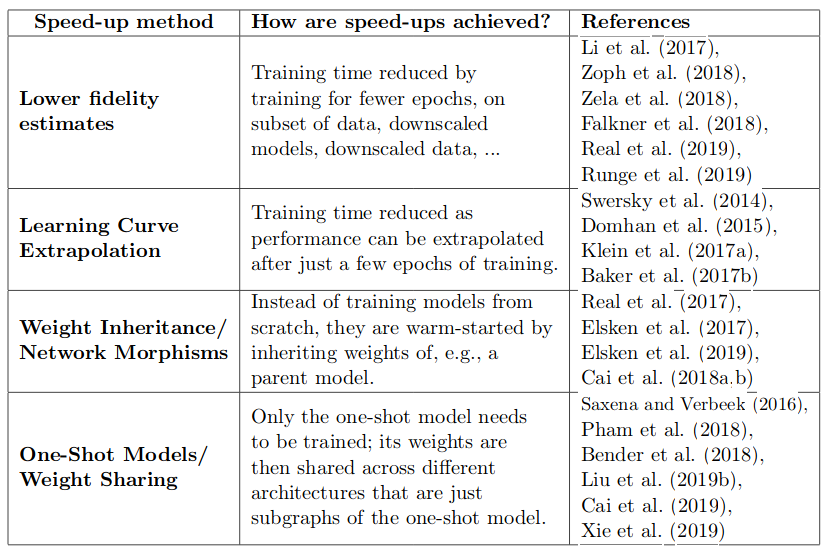
\includegraphics[width=0.9\textwidth]{images_lec7/performance_estimation.png}\\
\end{frame}
%----------------------------------------------------------------------



%----------------------------------------------------------------------
\begin{frame}[c]{Learning Goals}

After this lecture, you will be able to \ldots

\begin{itemize}
	\item describe \alert{several ways of speeding up over blackbox NAS}  %(except via meta-learning)
	\myit{
		\item define \alert{network morphisms} \& \alert{explain how to use them to speed up NAS}
		\item explain various \alert{methods for extrapolating learning curves}
		\item explain various \alert{multi-fidelity Bayesian optimization methods}
	}
	\item discuss \alert{when and how to use NAS and HPO in practice} 
	\myit{
		\item describe \alert{failure modes of DARTS}
		\item describe \alert{Auto-DispNet}
	} 
	\item describe \alert{NAS-Bench-101}, a benchmark for NAS
\end{itemize}

\end{frame}


%-----------------------------------------------------------------------
\section{Network Morphisms and Weight Inheritance}
%-----------------------------------------------------------------------


%----------------------------------------------------
\begin{frame}{Network Morphisms}
    \begin{itemize}
    	\item \alert{Network Morphisms} \lit{Chen et al. ‘16; Wei et al. ‘16; Cai et al. ‘17}
	\begin{itemize}
		\item[--] \alert{Change the network structure, but not the modelled function}
		\item[--] i.e., for every input the network yields the same output as before applying
		some network morphisms operations, such as ``Net2DeeperNet'', ``Net2WiderNet'', etc.
	\end{itemize}
    \end{itemize}

    \begin{figure}[t]
        \begin{centering}
            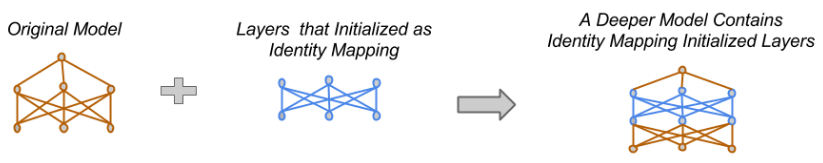
\includegraphics[scale=0.3]{images_lec7/net2deepernet.png}
        \end{centering}
    \end{figure}

\end{frame}

%----------------------------------------------------
\begin{frame}{Network Morphisms Allow Efficient Moves in Architecture Space}

    \begin{figure}[t]
        \begin{centering}
            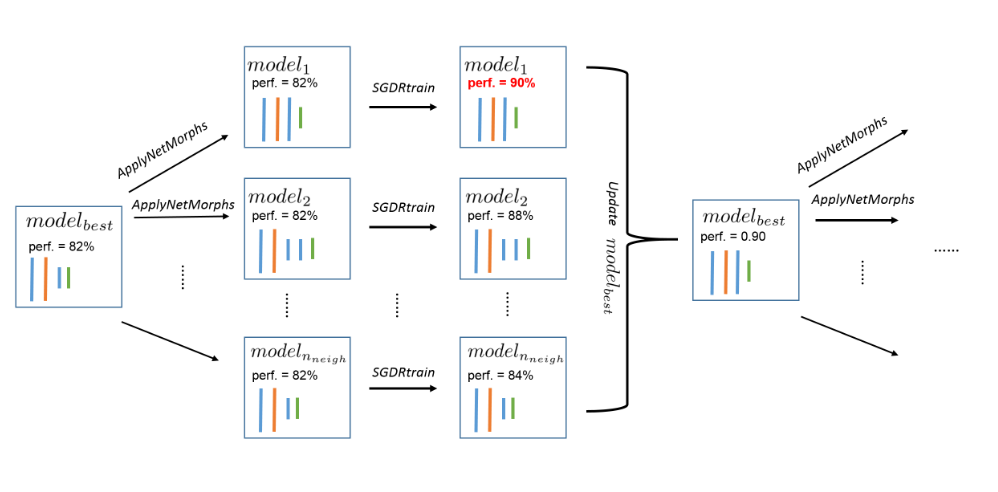
\includegraphics[scale=0.3]{images_lec7/NASH.png}
        \end{centering}
    \end{figure}


	%\alert{Weight Inheritance} 
	\lit{Real et al. ‘17; Cai et al, '17; Elsken et al, '17; Cai et al. ‘18; Elsken et al. ‘19}

\end{frame}
%----------------------------------------------------

%----------------------------------------------------
\begin{frame}{Efficient Multi-objective NAS \litw{Elsken et al. ‘19}}

{\small\alert{LEMONADE}: Lamarckian Evolution for Multi-Objective Neural Arch. Design}
    \begin{itemize}
    	\item Trades-off network size vs. performance
    	\myit{
    		\item Maintain a \alert{Pareto front} of the \alert{2 or more objectives}
			\item Evolve a population of Pareto-optimal architectures over time
		}
		\item Use \alert{weight inheritance}; no restriction to pure network morphisms
		\myit{
			\item[--] Inherit already trained weights from parent architectures to child ones
			\item[--] Do not necessarily require preserving the exact function
			\myit{
				\item \alert{approximate network morphisms}: function not perfectly preserved
			}
			\item[--] Still cheap through weight inheritance (1 week on 8 GPUs)
    	}

    \end{itemize}
\vspace*{-0.1cm}
    \begin{figure}[t]
        \begin{centering}
            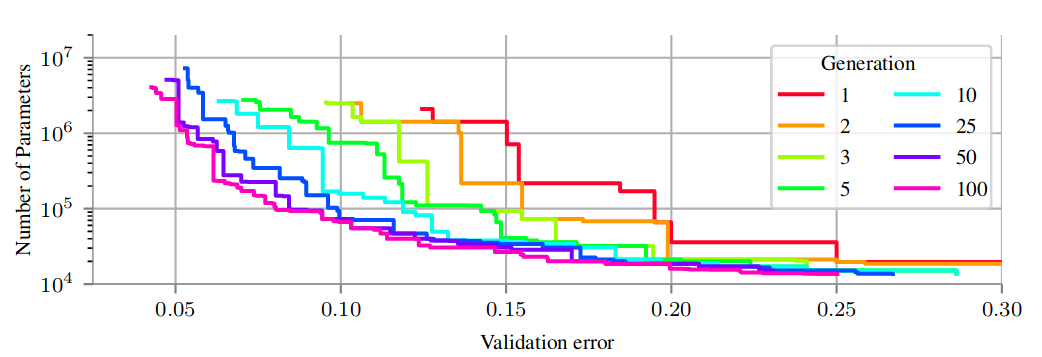
\includegraphics[scale=0.3]{images_lec7/lemonade.png}
        \end{centering}
    \end{figure}

\end{frame}
%----------------------------------------------------


%----------------------------------------------------

\begin{frame}[c]{Efficient Multi-objective NAS \litw{Elsken et al. ‘19}}
\begin{itemize}
	\item Children generation and training/evaluation of architectures 
\end{itemize}

\begin{centering}
    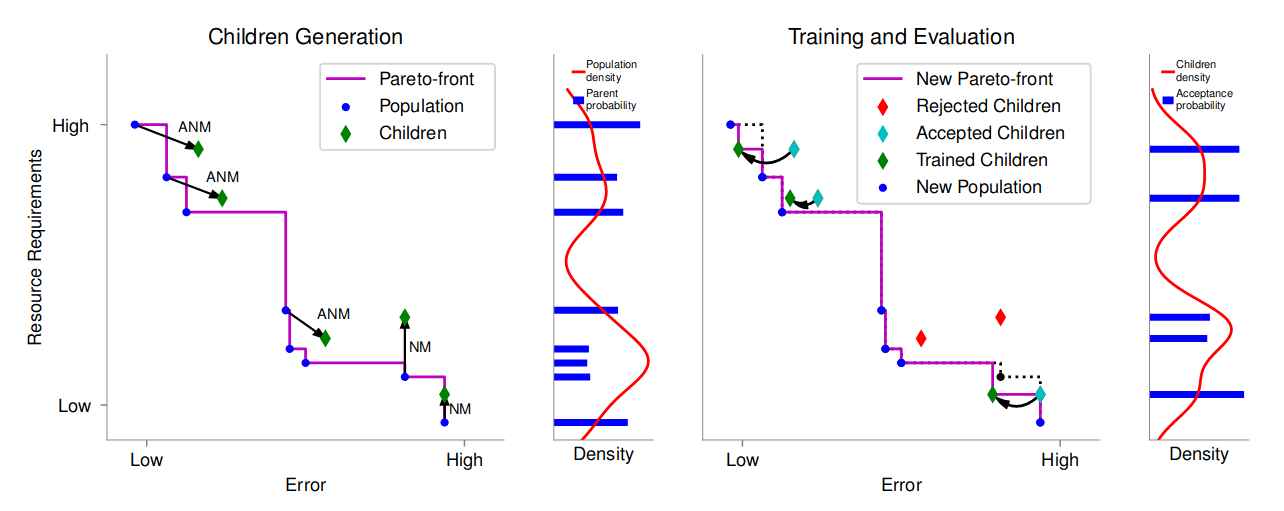
\includegraphics[scale=0.27]{images_lec7/lemonade_2.png}
\end{centering}

	\pause
	\myit{
			\item[--] \alert{Possible project: apply LEMONADE to SeizureNet}
			\item[--] \alert{Possible project: apply LEMONADE to algorithmic fairness}
			\item[--] \alert{Possible project: apply LEMONADE to adversarial robustness}
	}

\end{frame}

%----------------------------------------------------




%-----------------------------------------------------------------------
\section{Graybox Optimization: Learning Curve Extrapolation}
%----------------------------------------------------------------------

%-----------------------------------------------------------------------
\begin{frame}[c,fragile]{Learning Curves}

\centering
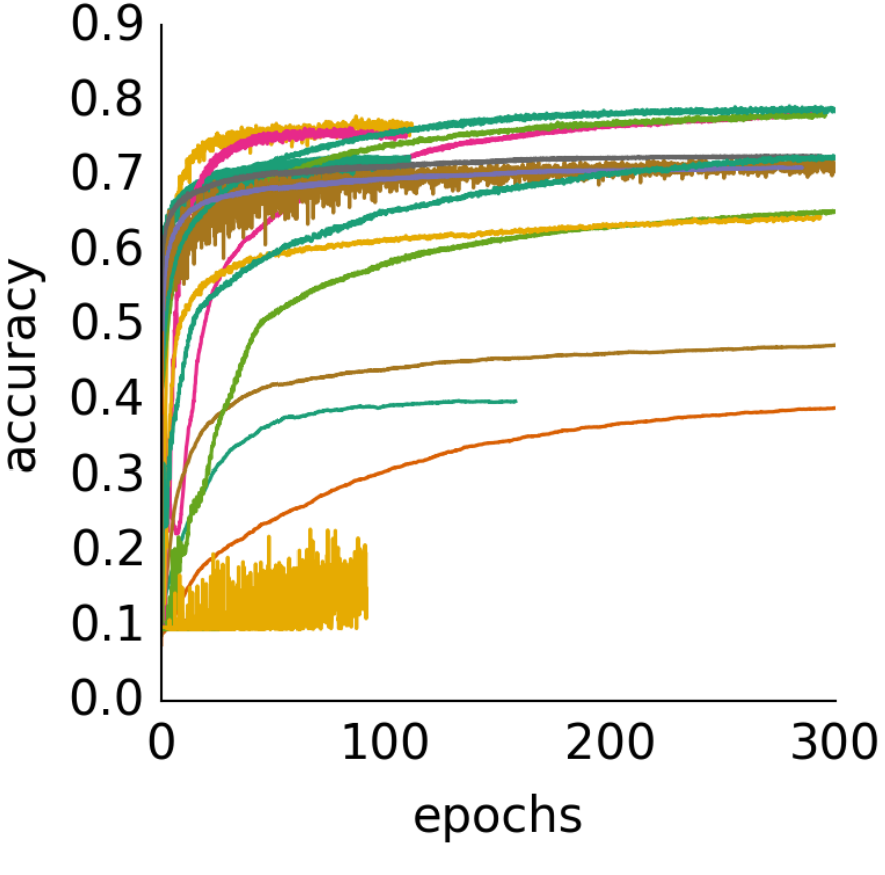
\includegraphics[width=0.5\textwidth]{images/learning_curves}

Exemplary learning curves of training deep neural networks\\
Many ML algorithms iteratively optimize a (loss) function

\end{frame}
%-----------------------------------------------------------------------

%-----------------------------------------------------------------------
\begin{frame}[c,fragile]{Learning Curve Predictions}

\centering
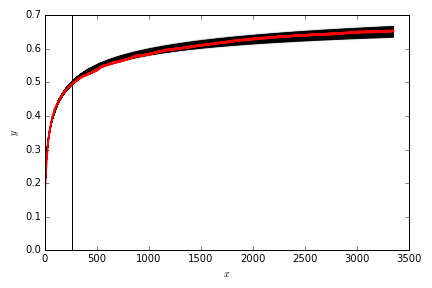
\includegraphics[width=0.6\textwidth]{images/learning_curve_single_pred}

\begin{enumerate}
  \item Observe learning curve for the first $n$ steps (here $n=250$)
  \pause
  \item \alert{Extrapolation}: fit parametric model on partial learning curve to predict remaining learning curve
  \pause
  \item Various models can be used (see following slides)
 % Which model to use? E.g.,
 % \begin{itemize}
%	\item Parametric density models: give table with equations
%	\item Neural network with learning curve layer
%	\item Recurrent neural network
%%    \item Good model depends on shape of curve $\to$ e.$\,$g., depends on optimizer  
%%    \item[$\leadsto$] combination of several models
%  \end{itemize}
  
\end{enumerate}

\end{frame}
%-----------------------------------------------------------------------

%-----------------------------------------------------------------------
\begin{frame}[c,fragile]{Learning Curves: Early Termination}

\centering
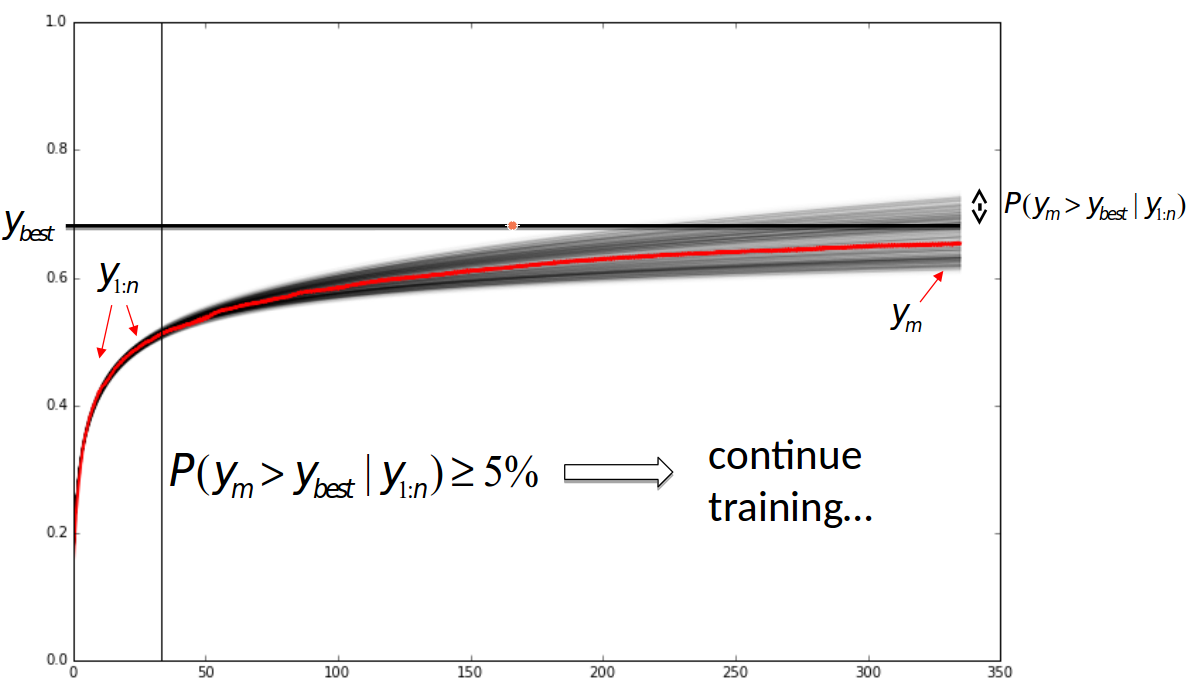
\includegraphics[width=\textwidth]{images/learning_curve_dec}

$\rightarrow$ need for probabilistic predictions / quantification of uncertainty

\end{frame}
%-----------------------------------------------------------------------
%-----------------------------------------------------------------------
\begin{frame}[c,fragile]{Learning Curves: Early Termination}

\centering
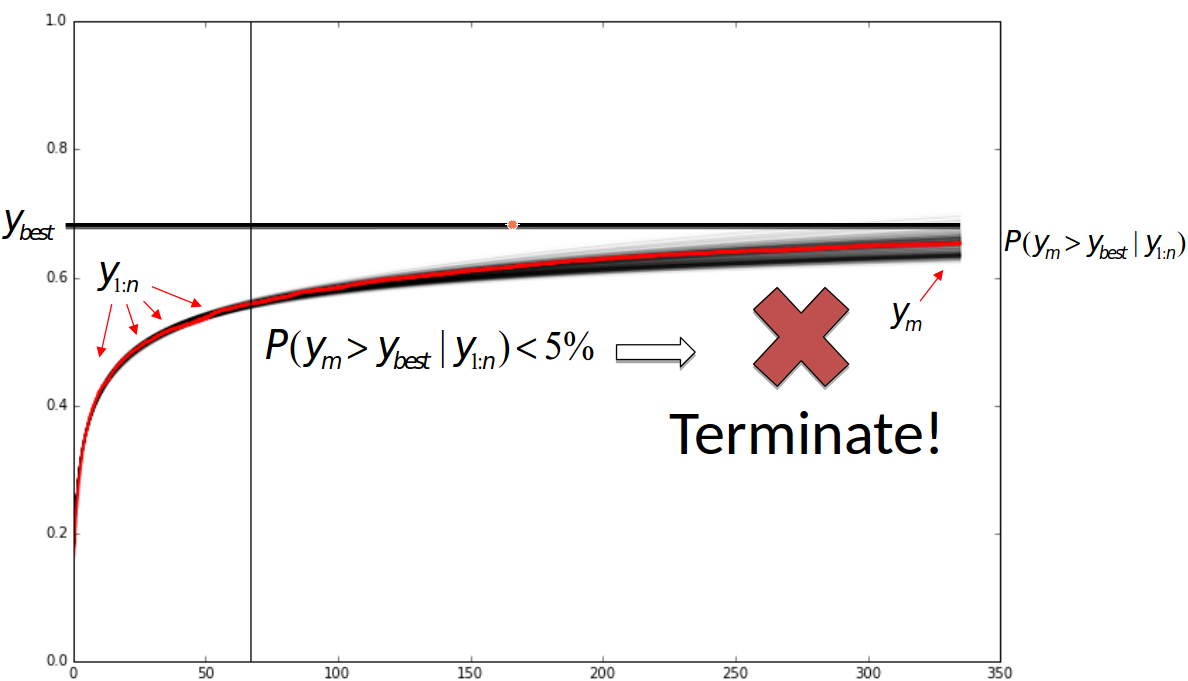
\includegraphics[width=\textwidth]{images/learning_curve_dec2}

$\rightarrow$ need for probabilistic predictions / quantification of uncertainty

\end{frame}
%-----------------------------------------------------------------------

%-----------------------------------------------------------------------
\begin{frame}[c,fragile]{Domhan et al, 2015: Parametric Learning Curves}

\myit{
	\item MSc Thesis in my group, 2015
	\item Use a parametric model $f_k$ with parameters $\boldsymbol{\theta}$ to model performance at step $t$ as:
	\alert{$y_t = f_k(t|\boldsymbol{\theta}) + \epsilon$}, with $\epsilon \sim \mathcal{N}(0, \sigma^2)$.
	\item Linear combination of $K=11$ parametric models:
	\alert{$f_{comb}(t|\bm{\xi}) = \sum_{k=1}^K w_k f_k(t|\boldsymbol{\theta}_k)$},
where $\bm{\xi} = (w_1, \dots, w_{K}, \boldsymbol{\theta}_1, \dots, \boldsymbol{\theta}_{K}, \sigma^2)$
}

\end{frame}
%-----------------------------------------------------------------------

%-----------------------------------------------------------------------
\begin{frame}[c,fragile]{Predictive Termination by Domhan et al, 2015}

\centering
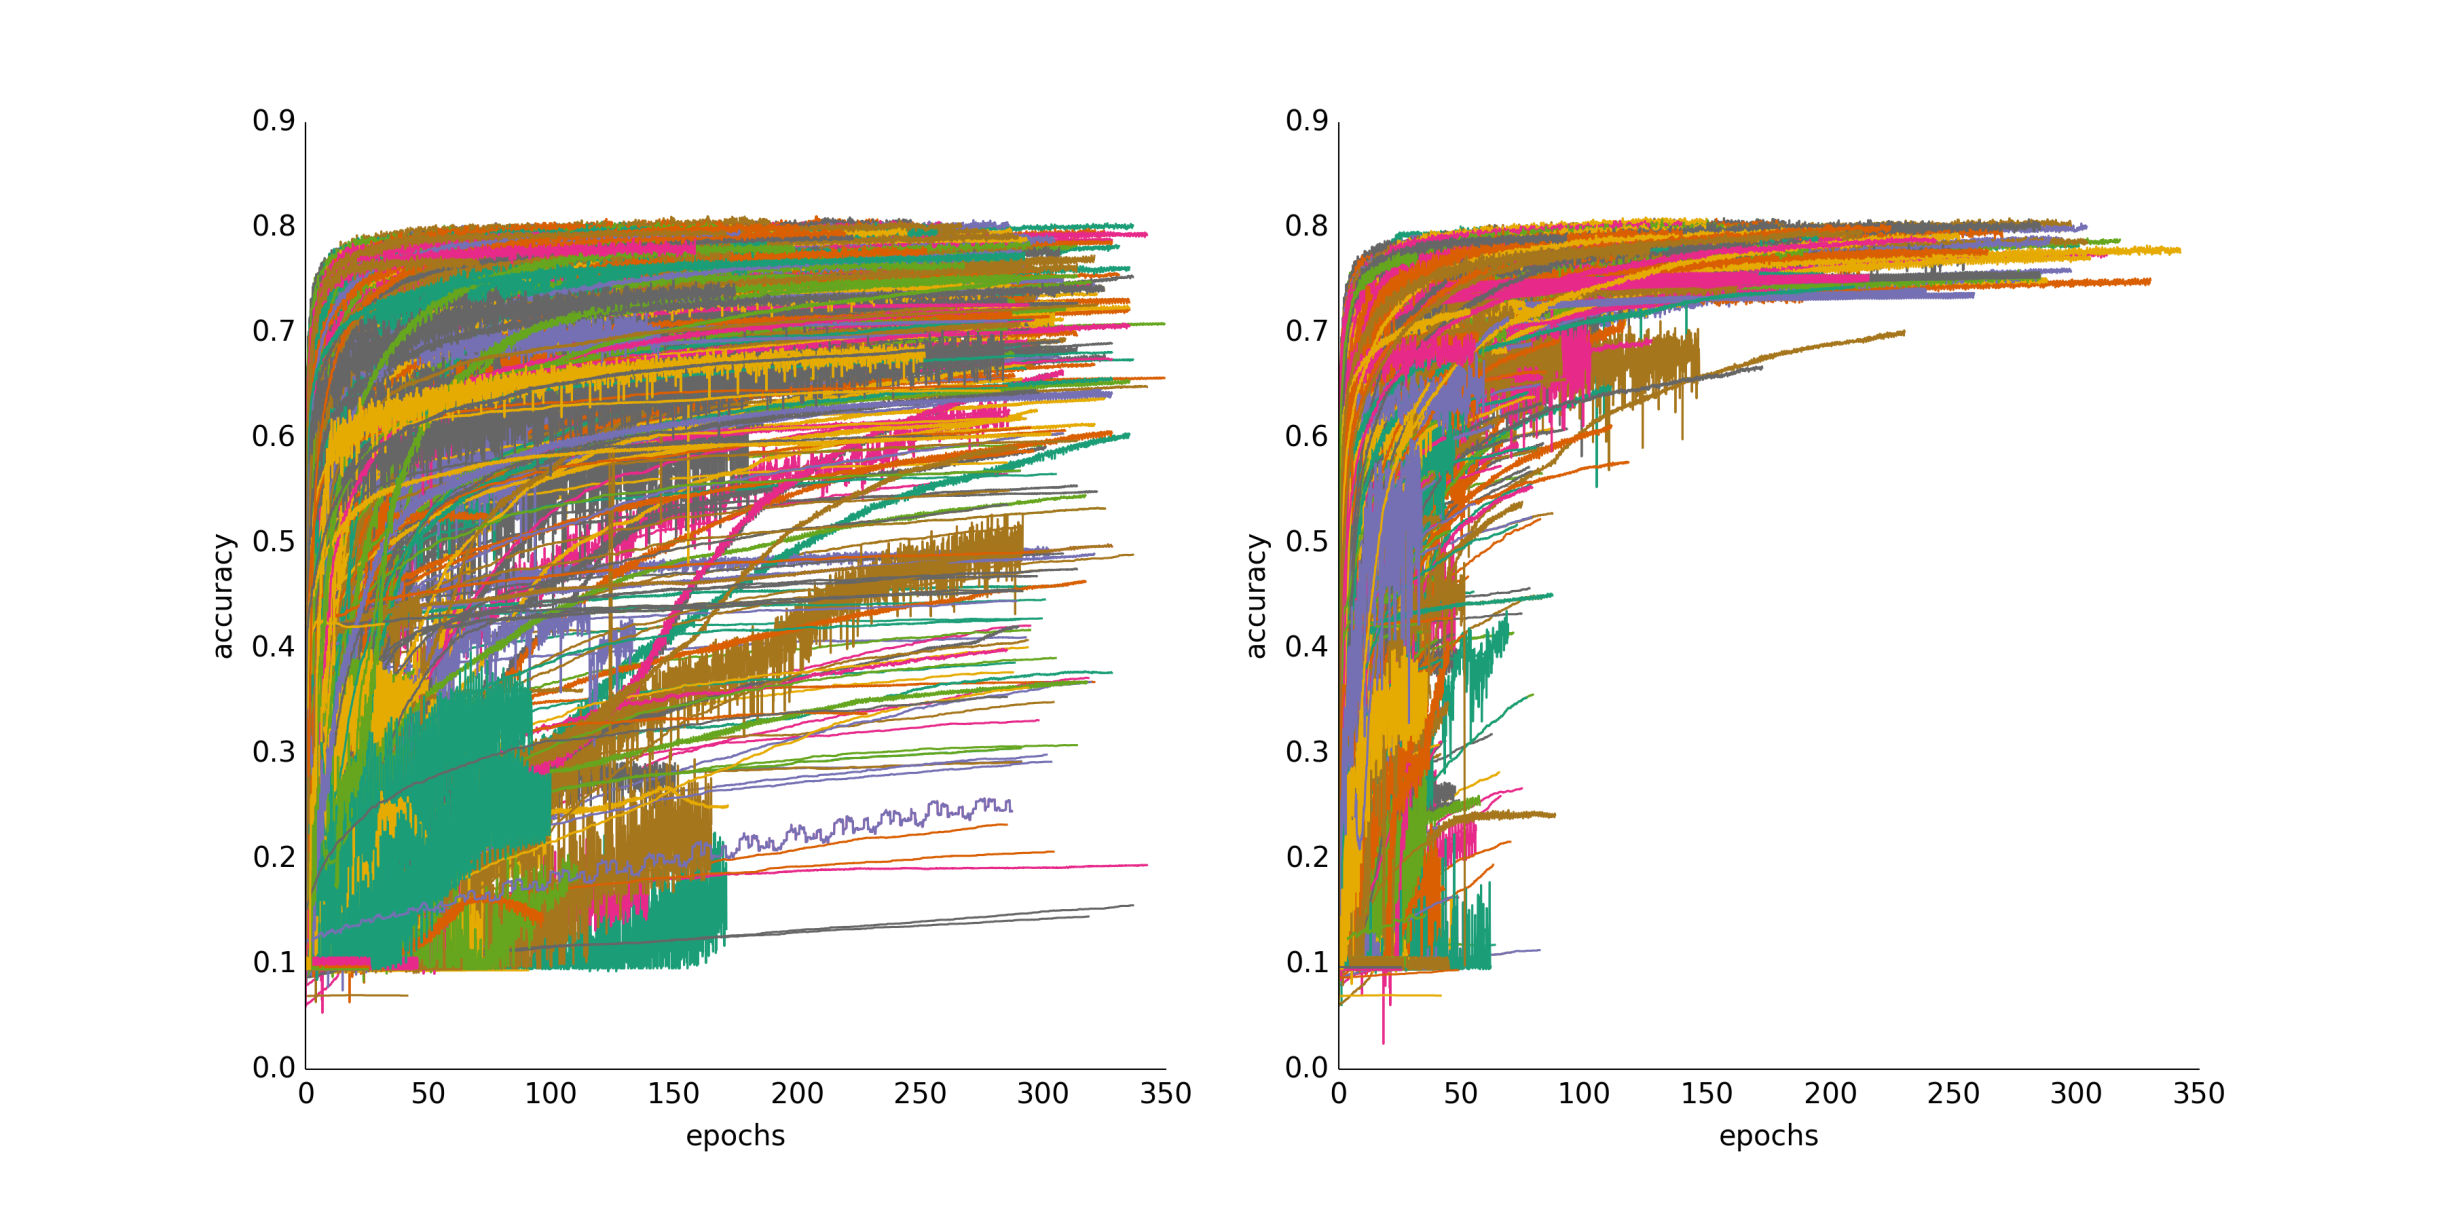
\includegraphics[width=\textwidth]{images/learning_curve_tuning}

All learning curves vs. learning curves with early termination
\pause

Disadvantages of this model? 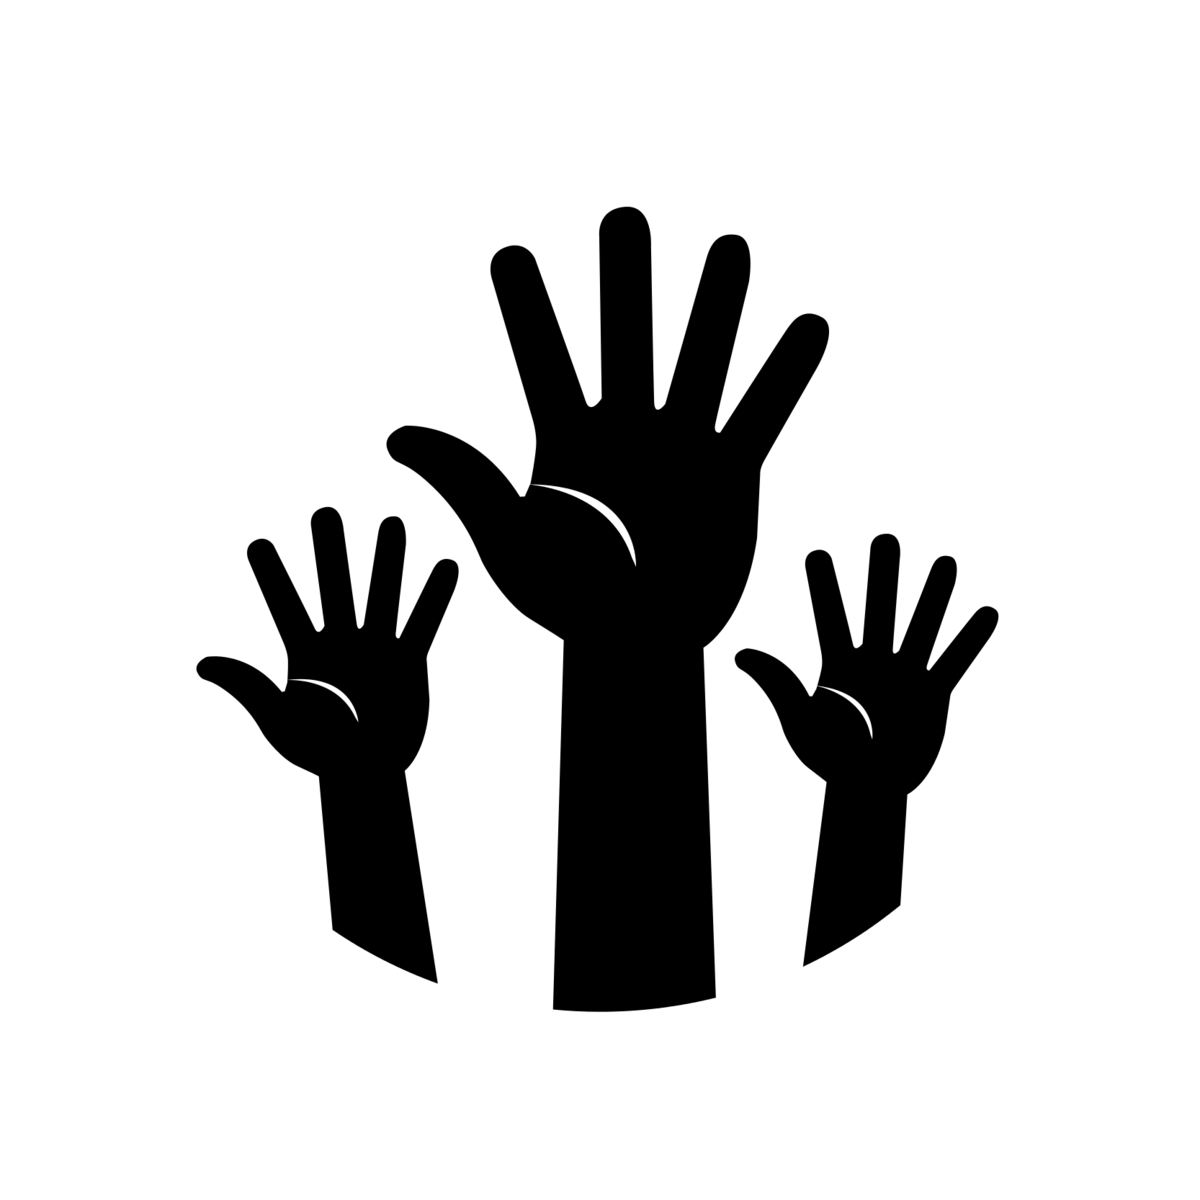
\includegraphics[height=0.1\textheight]{images/hands.png}

\end{frame}
%-----------------------------------------------------------------------


%-----------------------------------------------------------------------
\begin{frame}[c,fragile]{Klein et al, 2017: LC-Net}

TODO: copy figure

Disadvantages of this model? 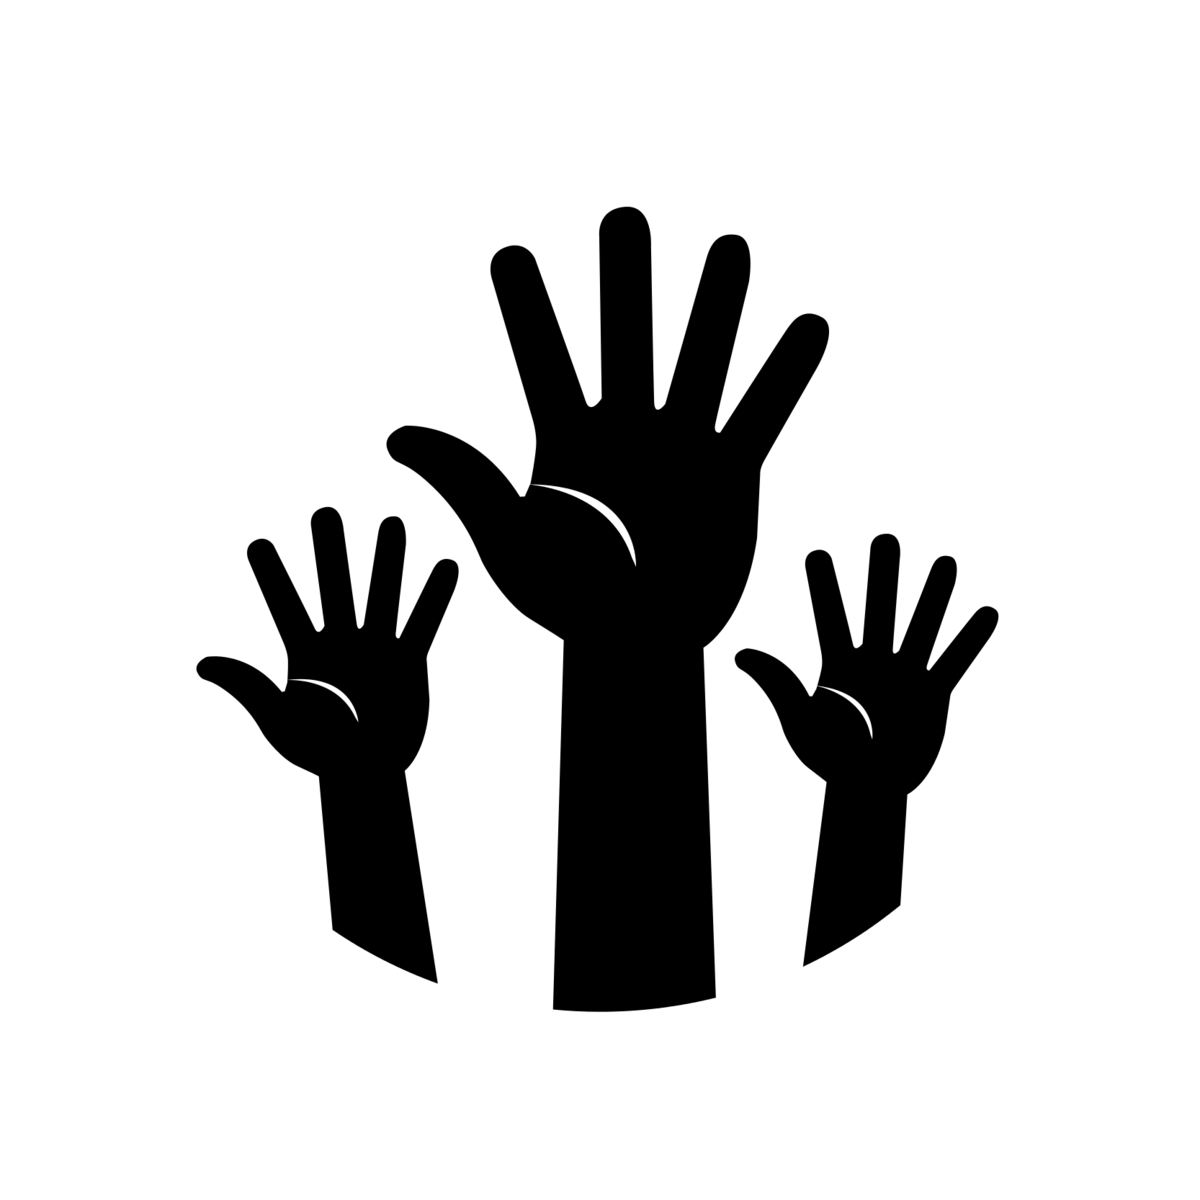
\includegraphics[height=0.1\textheight]{images/hands.png}

\end{frame}
%-----------------------------------------------------------------------



%-----------------------------------------------------------------------
\begin{frame}[c,fragile]{Gargiani et al, 2019: Sequence Model, e.g., Bayesian RNN}

TODO: copy figure; one of the formulas?


\end{frame}
%-----------------------------------------------------------------------

%-----------------------------------------------------------------------
\begin{frame}[c,fragile]{Compare: Baker et al, XXX}

Describe simple idea, and how that works extremely well when you have a budget of 10.000 of function evaluations.

\end{frame}
%-----------------------------------------------------------------------





%-----------------------------------------------------------------------
\section{Graybox Optimization: Using Multiple Fidelities}
%----------------------------------------------------------------------

TODO: can reuse slides from DL lecture last term?



%-----------------------------------------------------------------------
\myframe{Entropy search and KG}{
	\myit{
		\item About 5 slides, can maybe reuse parts from Peter
	}
}
%-----------------------------------------------------------------------


%-----------------------------------------------------------------------
\myframe{Some figures from Peter}{
	\myit{
		\item About 5 slides
		\item Mention the idea  
	}
}
%-----------------------------------------------------------------------

%-----------------------------------------------------------------------
\myframe{Generality of Multi-fidelity Methods}{
	\myit{
		\item \alert{Possible project: multi-multi-fidelity}
	}
}
%-----------------------------------------------------------------------

%-----------------------------------------------------------------------
\begin{frame}[c,fragile]{Subset Selection \litw{Klein et al. 2017}}

\begin{itemize}
  \item Problem: training is very slow for large datasets
  \item Idea: scaling up from subsets of data
  \item Example SVM:
  \begin{itemize}
    \item Computational cost grows quadratically in dataset size $s$
    \item Error shrinks smoothly with $s$
    \item Two parameters: $C$, $\lambda$
  \end{itemize}
\end{itemize}

\centering
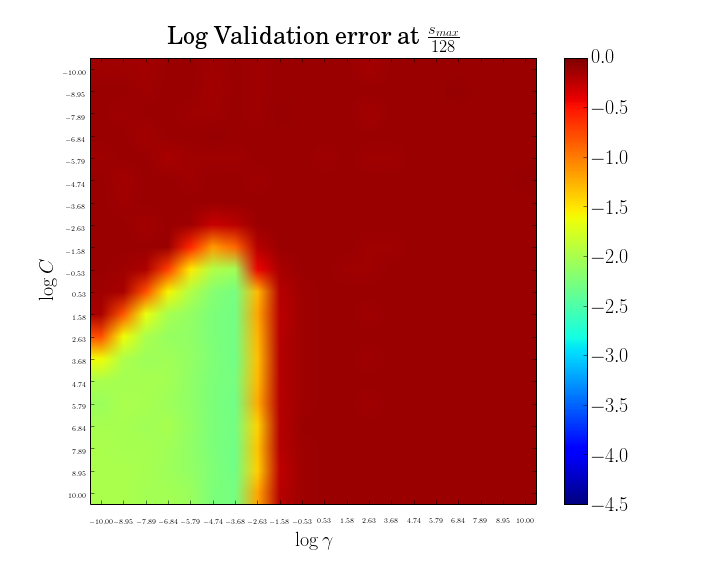
\includegraphics[width=0.28\textwidth]{images/subset_128}
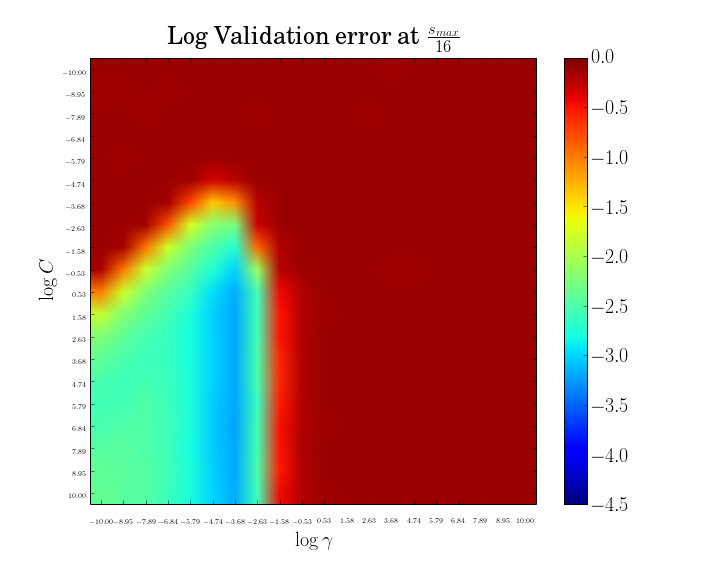
\includegraphics[width=0.28\textwidth]{images/subset_16}\\
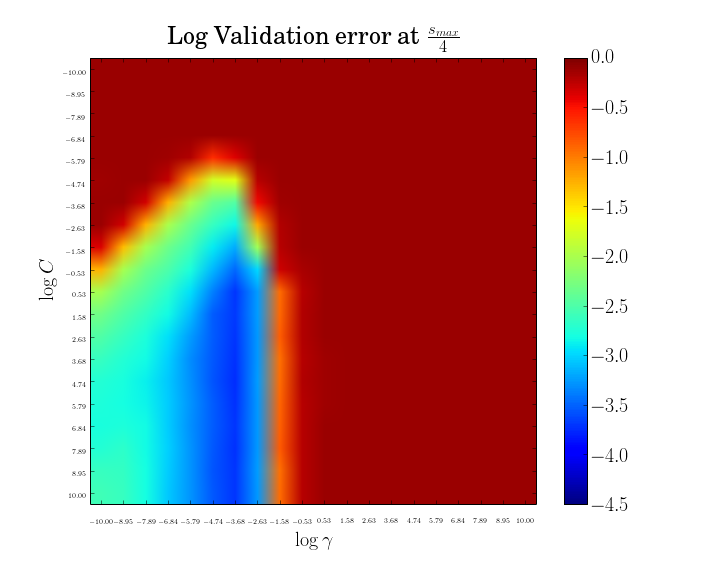
\includegraphics[width=0.28\textwidth]{images/subset_4}
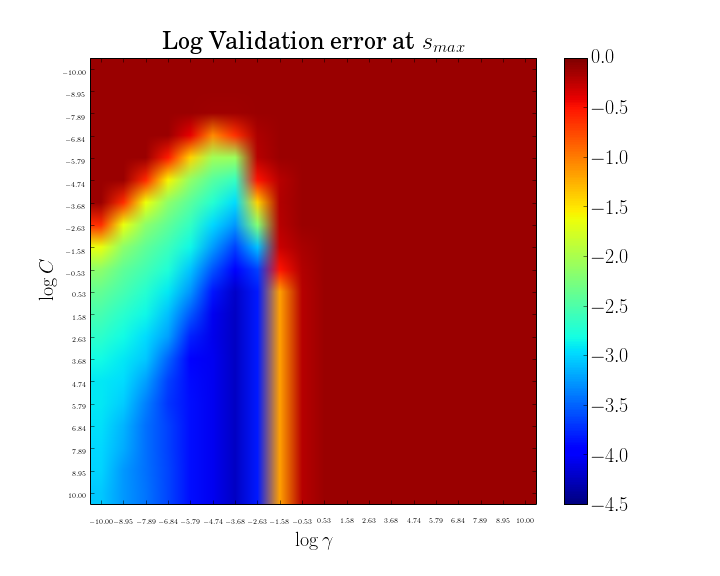
\includegraphics[width=0.28\textwidth]{images/subset_full}


\end{frame}
%-----------------------------------------------------------------------

%-----------------------------------------------------------------------
\begin{frame}[c,fragile]{Subset Selection \litw{Klein et al. 2017}}

\begin{itemize}
  \item Automatically choose dataset size for each evaluation
  \item Include extra dimension in probabilistic model to capture dependence on dataset size s: $f(\lambda,s)$
  \item Construct a second model for computational cost: $c(\lambda,s)$
  \item Trade off information gain about global optimum vs. cost
  \begin{itemize}
   \item Entropy Search \lit{Hennig \& Schuler, JMLR 2012}:\\ Based on a probability distribution of where the maximum lies
  \end{itemize} 
\end{itemize}

\centering
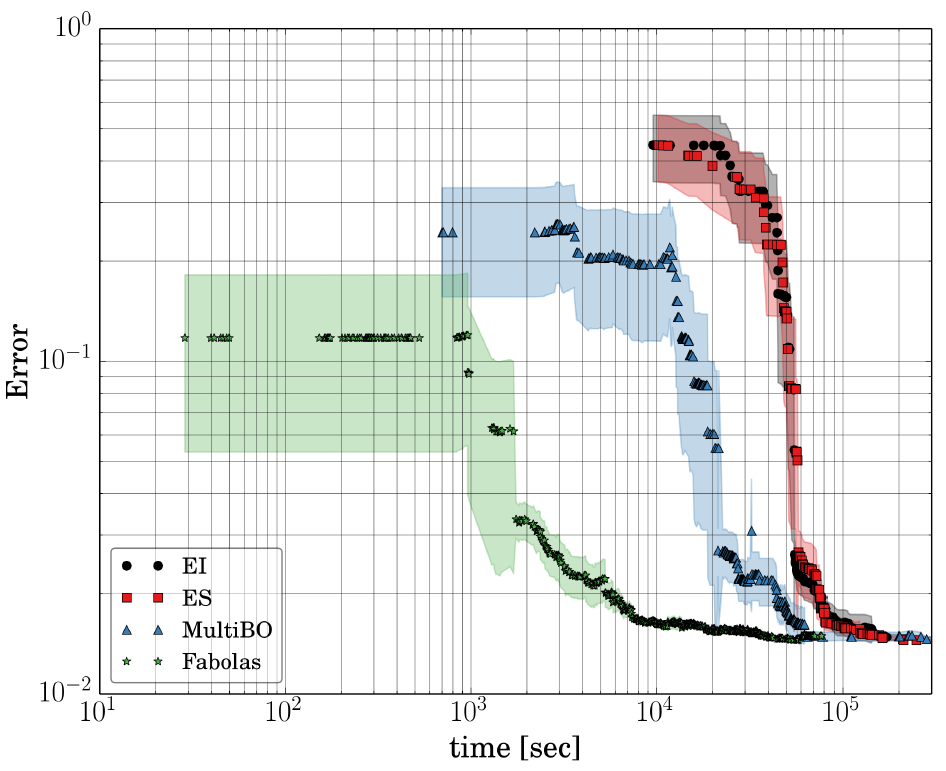
\includegraphics[width=0.4\textwidth]{images/subset_results}

\end{frame}
%-----------------------------------------------------------------------

%-----------------------------------------------------------------------
{\setbeamertemplate{logo}{}
\begin{frame}[c,fragile]{Successive Halving \litw{Jamieson and Talwalkar 2015}}

\begin{block}{Successive Halving}
\begin{itemize}
  \item Ideas: 
  \begin{itemize}
    \item Invest only resources in promising configurations
    \item[$\leadsto$] aggressive dropping of poor configurations
    \item Model-free --- (more or less assumption free)
  \end{itemize}
  \pause
  \item Algorithm Outline:
  \begin{enumerate}
    \item[-] Input: $n$ (randomly sampled) configurations and budget $B$
    \pause
    \item Run remaining configurations with some resource allocation\\ (depending on $B$)
    \pause
    \item Sort configurations by cost (e.$\,$g., validation loss)
    \item Throw away lower half of configurations
    \pause
    \item Repeat
  \end{enumerate}
  \pause
  \item Resource allocation can correspond to
  \begin{itemize}
    \item partial learning curves
    \item subset of training data
  \end{itemize}
\end{itemize}
\end{block}

\end{frame}
}
%-----------------------------------------------------------------------
%-----------------------------------------------------------------------
{\setbeamertemplate{logo}{}
\begin{frame}[c,fragile]{Hyperband \litw{Li et al. 2016}}

\begin{block}{Hyperband}
\begin{itemize}
  \item Issue of successive halving (for a fixed $B$):\\
  		Do you want to run many configurations with aggressive rejection?\\
  		Or: Do you want to run few configurations with non-aggressive rejection? 
  \pause
  \item Ideas: 
  \begin{itemize}
    \item Add an outer loop to try different trade-offs between $\#$configurations and budget
    \item Add further parameter: proportion of configurations discarded in each round of successive halving
  \end{itemize}
  \pause
  \item Starts with many configurations that gets aggressively rejected
  \pause
  \item In later iterations, few configurations with more budget each
  \pause
  \item Returns: configuration with the smallest intermediate loss seen so far.
\end{itemize}
\end{block}

\end{frame}
}
%-----------------------------------------------------------------------
%-----------------------------------------------------------------------
\begin{frame}[c,fragile]{Random Search vs. Hyperband}

\centering
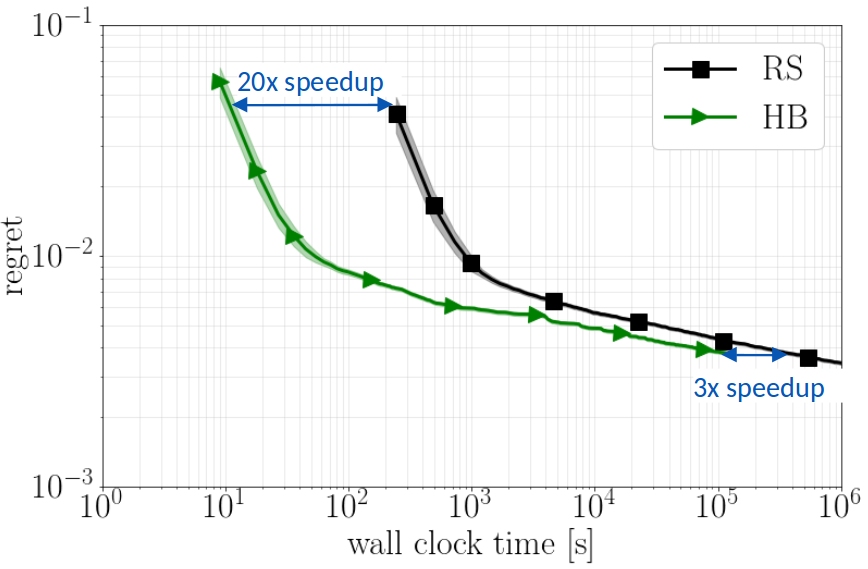
\includegraphics[width=0.8\textwidth]{images/randomsearch_hyperband}

\end{frame}
%-----------------------------------------------------------------------
%-----------------------------------------------------------------------
\begin{frame}[c,fragile]{Random Search vs. Bayesian Optimization}

\centering
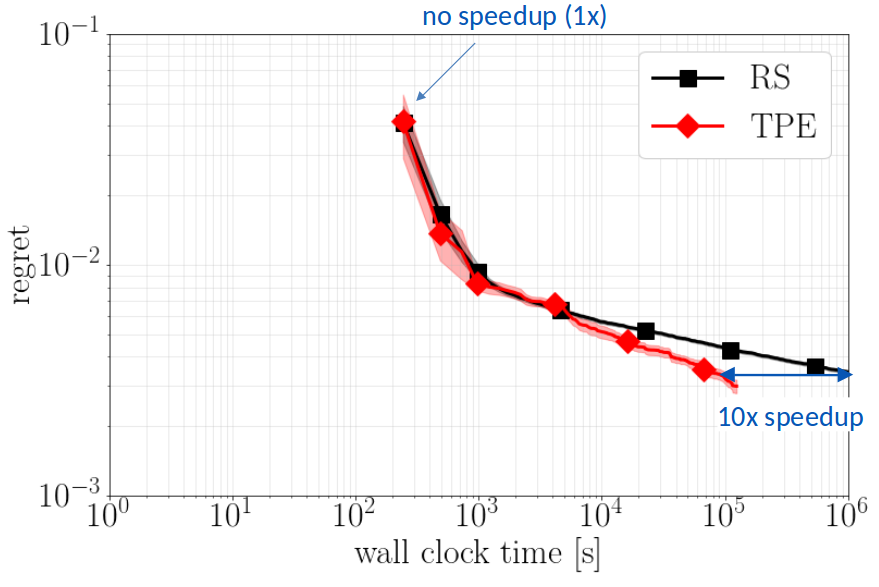
\includegraphics[width=0.8\textwidth]{images/randomsearch_bo}

\end{frame}
%-----------------------------------------------------------------------
%-----------------------------------------------------------------------
\begin{frame}[c,fragile]{Random Search vs. Bayesian Optimization vs. BOHB}

\centering
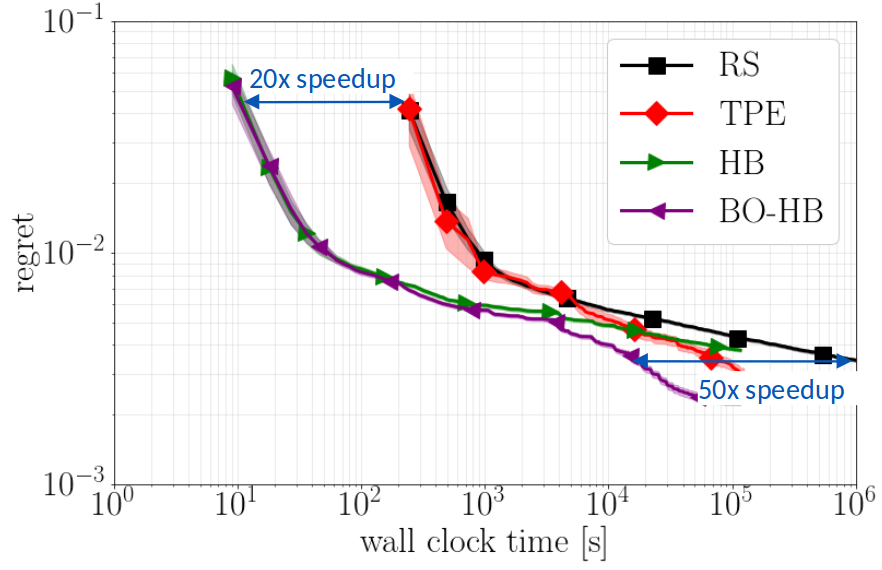
\includegraphics[width=0.8\textwidth]{images/randomsearch_bohb}

\end{frame}
%----------------------------------------------------------------------



%-----------------------------------------------------------------------
\section{Case Study: Auto-DispNet}
%-----------------------------------------------------------------------


%----------------------------------------------------------------------
\myframe{The Problem of Disparity Estimation}{
	\myit{
		\item .
	}	
}
%----------------------------------------------------------------------

%----------------------------------------------------------------------
\myframe{Background: U-Net}{
	\myit{
		\item Skip connections from same spatial resolution to avoid loosing information
	}	
}
%----------------------------------------------------------------------

%----------------------------------------------------------------------
\myframe{Search space 1/2}{
	\myit{
		\item Standard cells like in DARTS for 
		\myit{
			\item Keeping spatial resolution
			\item Downsampling
		}
	}	
}
%----------------------------------------------------------------------

%----------------------------------------------------------------------
\myframe{Search space 2/2}{
	\myit{
		\item New upsampling cell that supports U-Net like skip connections 
	}	
}
%----------------------------------------------------------------------

%----------------------------------------------------------------------
\myframe{Neural Architecture Search by DARTS, HPO by BOHB}{
	\myit{
		\item Both components contributed substantially:
		\myit{
			\item a
			\item b
		} 
	}	
}
%----------------------------------------------------------------------

%----------------------------------------------------------------------
\myframe{Details for Neural Architecture Search by DARTS}{
	\myit{
		\item Performance improved substantially
		\item Very important: \alert{warmstarting} of the network weights
		\myit{
			\item First, keep one-shot architecture weights fixed to the uniform distribution
			\item Only afterwards, alternative updates of weights and architectural parameters
		}
		\item Without warmstarting: \alert{DARTS found cells with only parameterless operations}
	}	
}
%----------------------------------------------------------------------

%----------------------------------------------------------------------
\myframe{Failure Modes of DARTS}{
	\myit{
		\item Idenfified six small search spaces where DARTS fails badly.
		\item Show plots
	}	
}
%----------------------------------------------------------------------

%----------------------------------------------------------------------
\myframe{Failure Modes of DARTS}{
	\myit{
		\item Show analysis
	}	
}
%----------------------------------------------------------------------

%----------------------------------------------------------------------
\myframe{Failure Modes of DARTS}{
	\myit{
		\item Show countermeasures.
	}	
}
%----------------------------------------------------------------------










%-----------------------------------------------------------------------
\myframe{NAS-Bench-101}{
	\myit{
		\item About 5 slides on this, in the end, after explaining BOHB etc.
		\item Mention ideas for Nas-Bench-102
		\item Mention plans for HPOlib 2.0
	}
}
%-----------------------------------------------------------------------

%-----------------------------------------------------------------------
\myframe{Robustifying DARTS}{
	\myit{
		\item Show all the bad failure modes of DARTS
		\item Go through that paper; 5 slides
	}
}
%-----------------------------------------------------------------------

%-----------------------------------------------------------------------
\myframe{Auto-DispNet}{
	\myit{
		\item Go through that paper; 5 slides
		\item Optimization by BOHB
	}
}
%-----------------------------------------------------------------------


%-----------------------------------------------------------------------
\myframe{}{
	\myit{
		\item a
	}
}
%-----------------------------------------------------------------------

%-----------------------------------------------------------------------
\myframe{}{
	\myit{
		\item a
	}
}
%-----------------------------------------------------------------------


%-----------------------------------------------------------------------
\begin{frame}[c,fragile]{What if a single configuration is too expensive?}


\begin{itemize}
  \item Sometimes, even validating a single configuration needs a lot of time\\
  		e.$\,$g., single function evaluation takes hours or even days:
  \begin{itemize}
    \item ML on big data
    \item Training a deep neural network  
  \end{itemize}
  \pause
  \item Challenge: We cannot search for a configuration if we can afford very few function evaluations $< 10$
  \pause
  \item \hands What could we do?
  \pause
  \begin{itemize}
    \item Data subset selection
    \item Predict learning curves
  \end{itemize}
  \item[$\leadsto$] Going from black-box to grey-box optimization
\end{itemize}

\end{frame}
%-----------------------------------------------------------------------

